
\documentclass[times, 10pt,twocolumn]{article} 
%\documentclass[times, 12pt]{article} 

\usepackage{geometry} % See geometry.pdf for lots of layout options. 
\usepackage{graphicx}
\usepackage{amssymb}
\usepackage{subfigure}
\usepackage{cite}
\usepackage{hyphenat}
\usepackage{latex8}
\usepackage{times}
% \usepackage{setspace}

\newbox\subfigbox % Create a box to hold the subfigure. 
\makeatletter 
\newenvironment{subfloat}% % Create the new environment. 
{\def\caption##1{\gdef\subcapsave{\relax##1}}% 
\let\subcapsave=\@empty % Save the subcaption text. 
\let\sf@oldlabel=\label 
\def\label##1{\xdef\sublabsave{\noexpand\label{##1}}}% 
\let\sublabsave\relax % Save the label key. 
\setbox\subfigbox\hbox 
\bgroup}% % Open the box... 
{\egroup % ... close the box and call \subfigure. 
\let\label=\sf@oldlabel 
\subfigure[\subcapsave]{\box\subfigbox}}% 
\makeatother 

% \doublespacing


\title{FlatCAD and FlatLang: Kits by Code} 

\author{
Gabe Johnson\\
Carnegie Mellon University
}

\begin{document}

 \maketitle


\begin{abstract}
The \nohyphens{FlatCAD} system lets you create your own physical
construction kits by coding in the LOGO-like \nohyphens{FlatLang}
language. No longer must construction kit pieces be merely a product
designed by someone else: if you can write a simple
\nohyphens{FlatLang} program, you can design a kit. This paper
describes our domain-specific language features and example output.
\end{abstract}

\section{Introduction}

Construction kits let you build complex things using simple pieces. A
typical set of LEGO bricks consist of plastic pieces that snap
together vertically. Another popular kit, Tinker Toys, features rigid
struts that fit into round holes in hubs. Many more examples can be
found at toy stores. Most kits present different types of pieces that
vary in size, length, or the way they fit together. Despite (or
perhaps because of) the kits' simplicity, they support people in
building creative, complex constructions.

In existing kits, individual pieces are immutable. But what if we
could design new kinds of parts? Instead of building from the parts we
are given, we could instead make new kinds of kits that enable us to
work in different ways. To explore this question, we have developed
\nohyphens{FlatCAD}, a prototype system that supports user who wish to
develop new kinds of construction kits.

Our system is intended for helping people design and fabricate
construction kits and models using rapid prototyping machines. The
price of this machinery continues to drop as quality improves. Soon
most elementary schools will have prototyping machines such as 3D
printers and laser cutters. However, the usefulness of these machines
is limited by the available software to design for
fabrication. Current CAD software is made for professional designers
and its complexity renders it largely inaccessible to people.

Traditional kits are the toys of the era of mass production. Rapid
prototyping machines and appropriate design software lets us make new
kinds of kits in an era of mass customization. With
\nohyphens{FlatCAD}, we can write programs that not only produce
graphics but customized physical output as well.

\nohyphens{FlatCAD} is a design system for modeling and fabricating 3D
objects using flat material like wood, acrylic, paper, or
cardboard. These materials may be \underline{f}olded,
\underline{l}ayered, \underline{a}ttached, and \underline{t}rimmed in
various ways to create physical constructions---hence ``flat''
CAD. These models can then be `printed' to rapid prototyping devices
such as laser cutters for manual
assembly. Figure~\ref{fig:physical-output} shows examples of models
and kits made with \nohyphens{FlatCAD}.

Users make \nohyphens{FlatCAD} models by programming in a LOGO-like
scripting language called \nohyphens{FlatLang}. It allows users to
quickly create shapes by experimenting with code, bringing the power
of programming to bear on the process of making physical artifacts. To
illustrate this, in the following section we show how people can
design and construct a class of simple mechanical automata using
\nohyphens{FlatCAD}.

\begin{figure}
   \centering
   \subfigure[Parametric boxes whose faces attach with finger joints.] {
     \label{fig:physical-output-boxcad}
     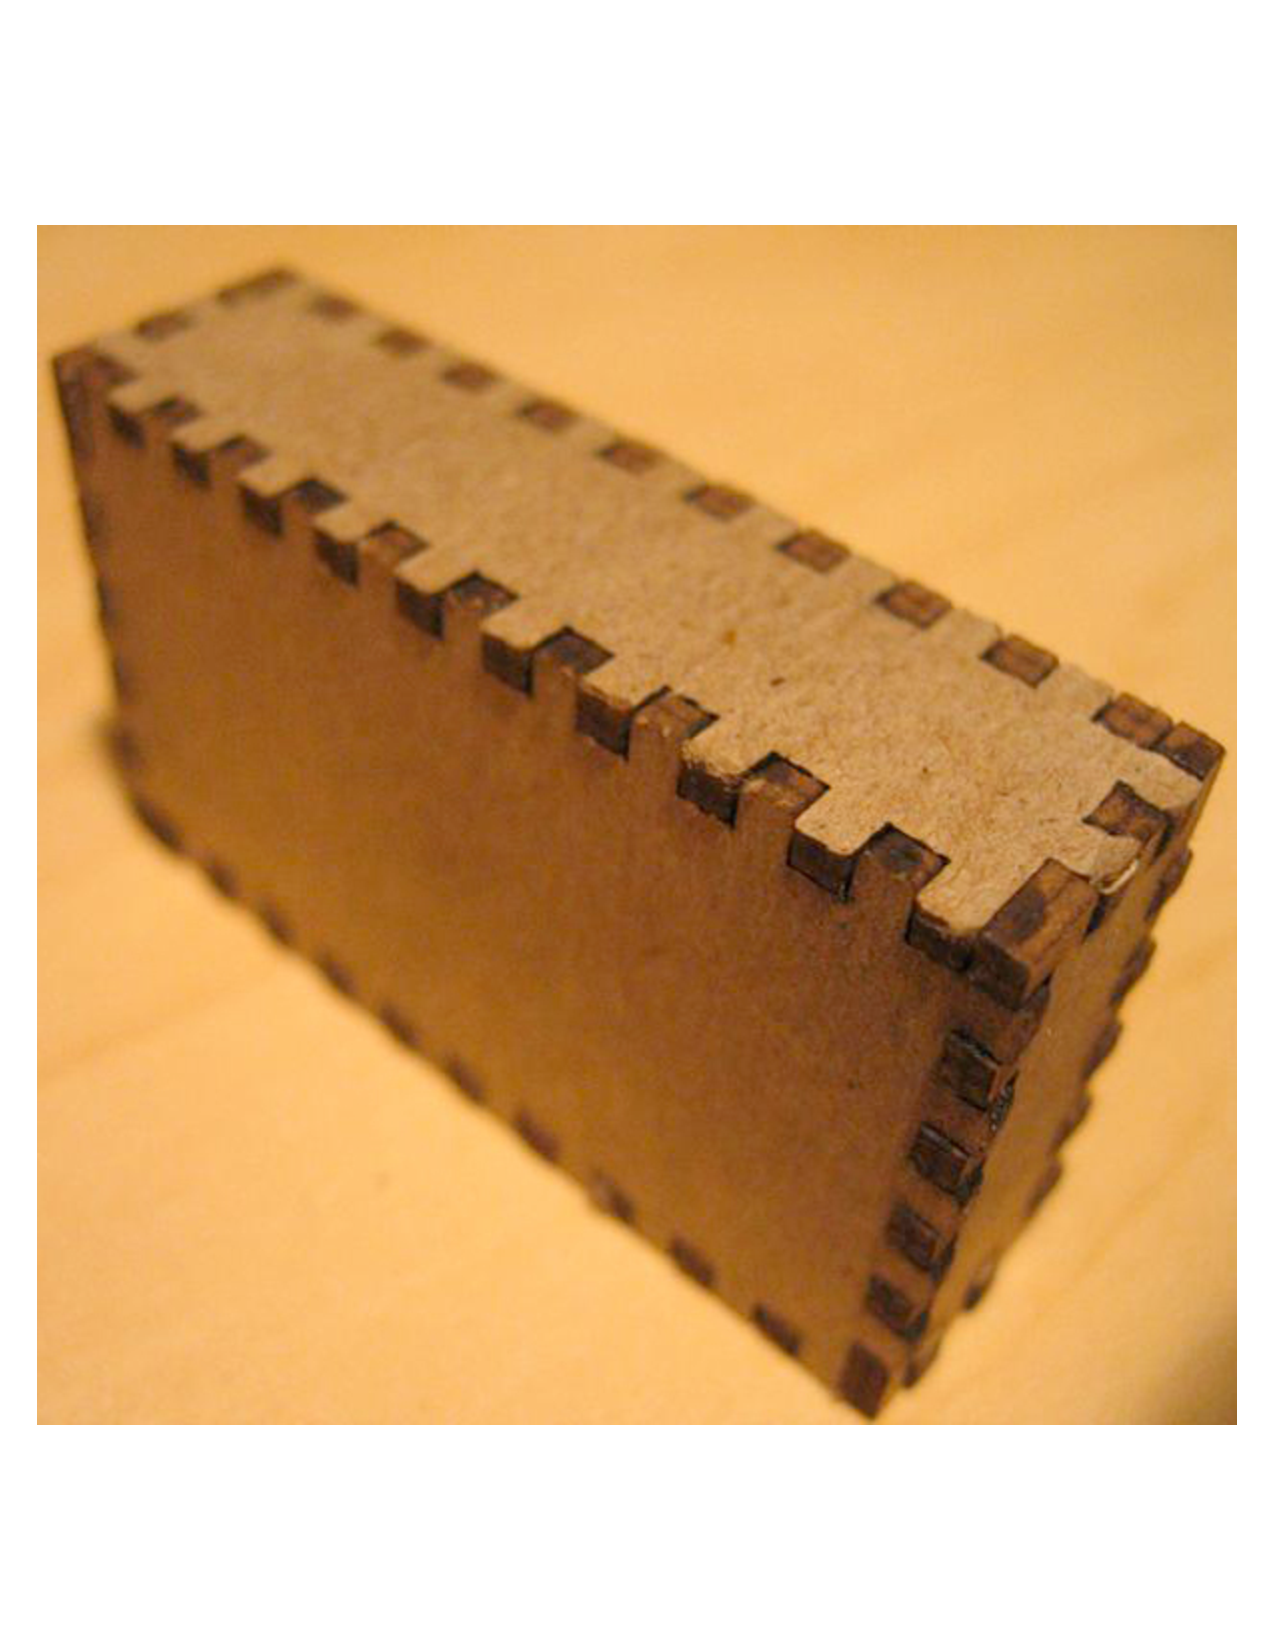
\includegraphics[width=0.9in]{physical-output-boxcad.pdf}
   }
   \hspace{2mm}
   \subfigure[A simple kit with notched pieces.] {
     \label{fig:physical-output-jessica}
     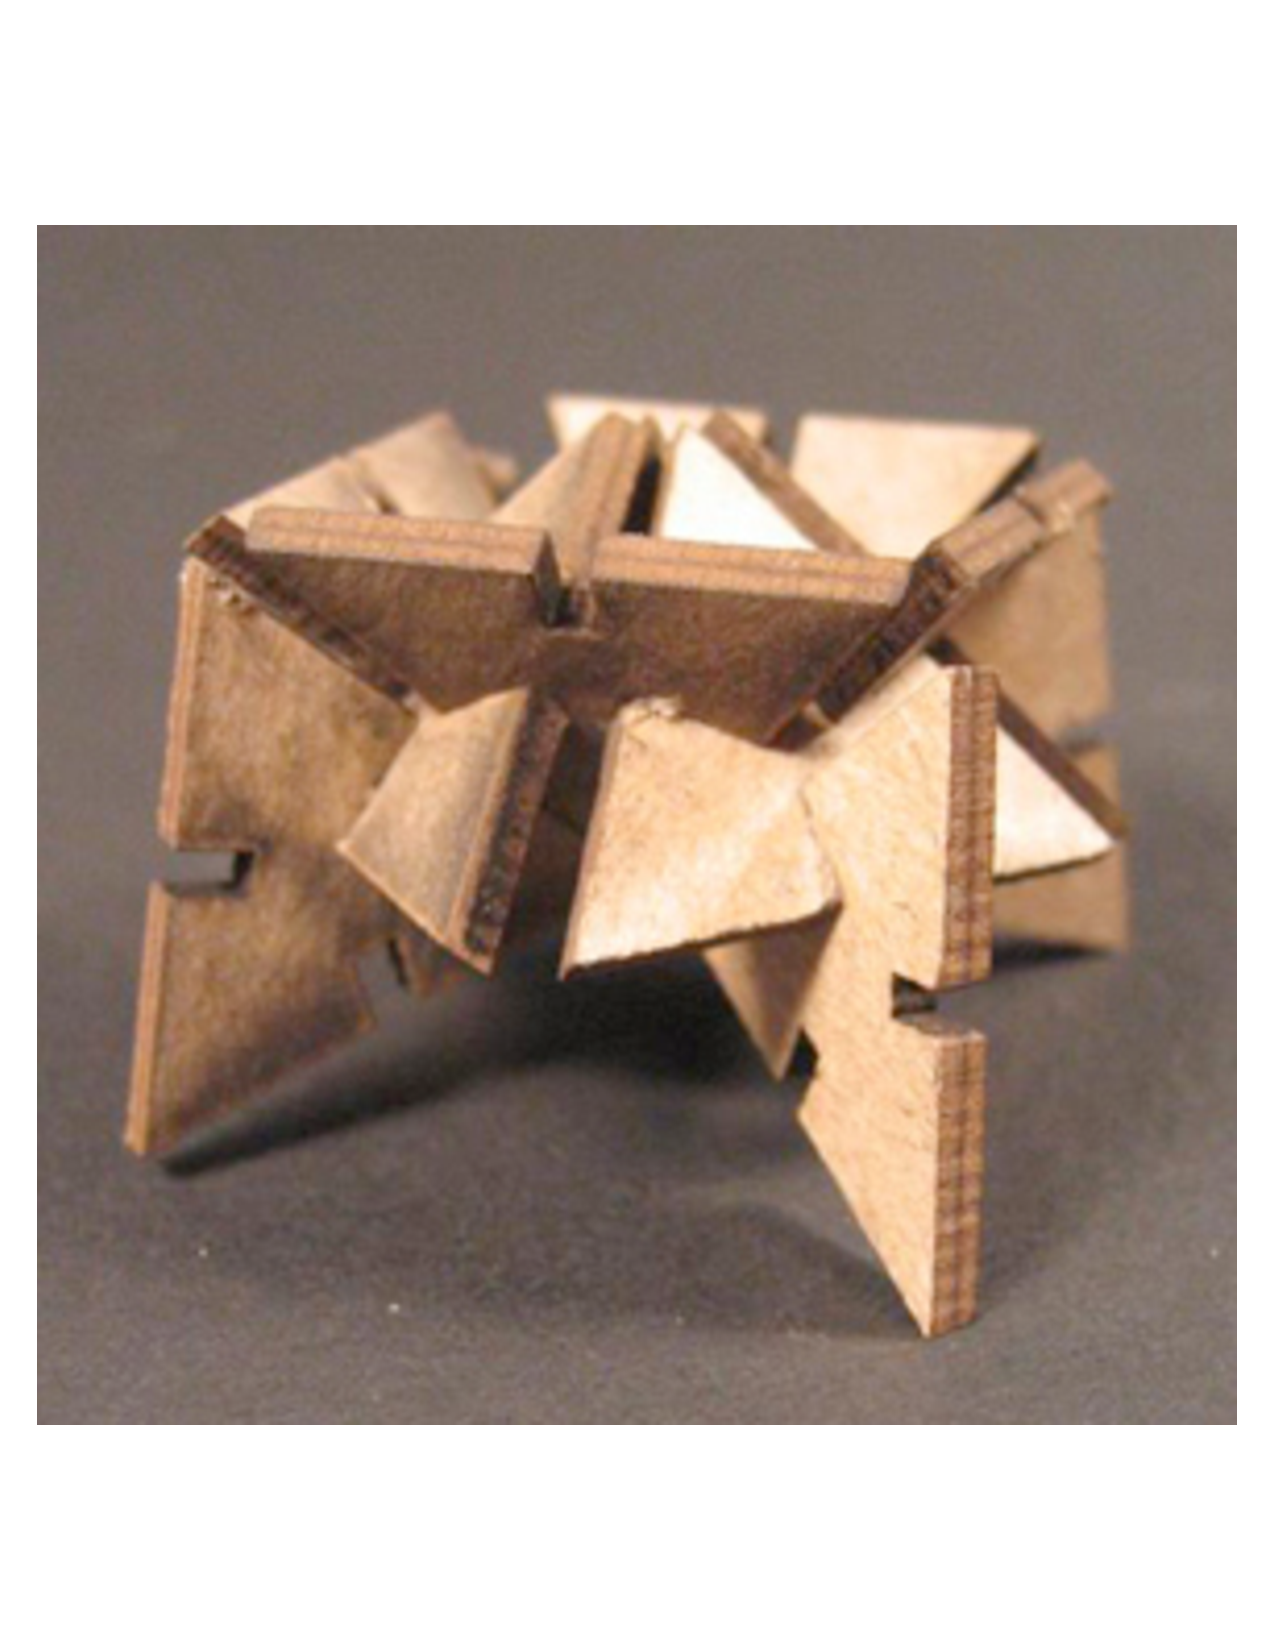
\includegraphics[width=0.9in]{physical-output-jessica.pdf}
   }
   \hspace{2mm}
   \subfigure[Gears are one type of piece in mechanical kits.] {
     \label{fig:physical-output-gears}
     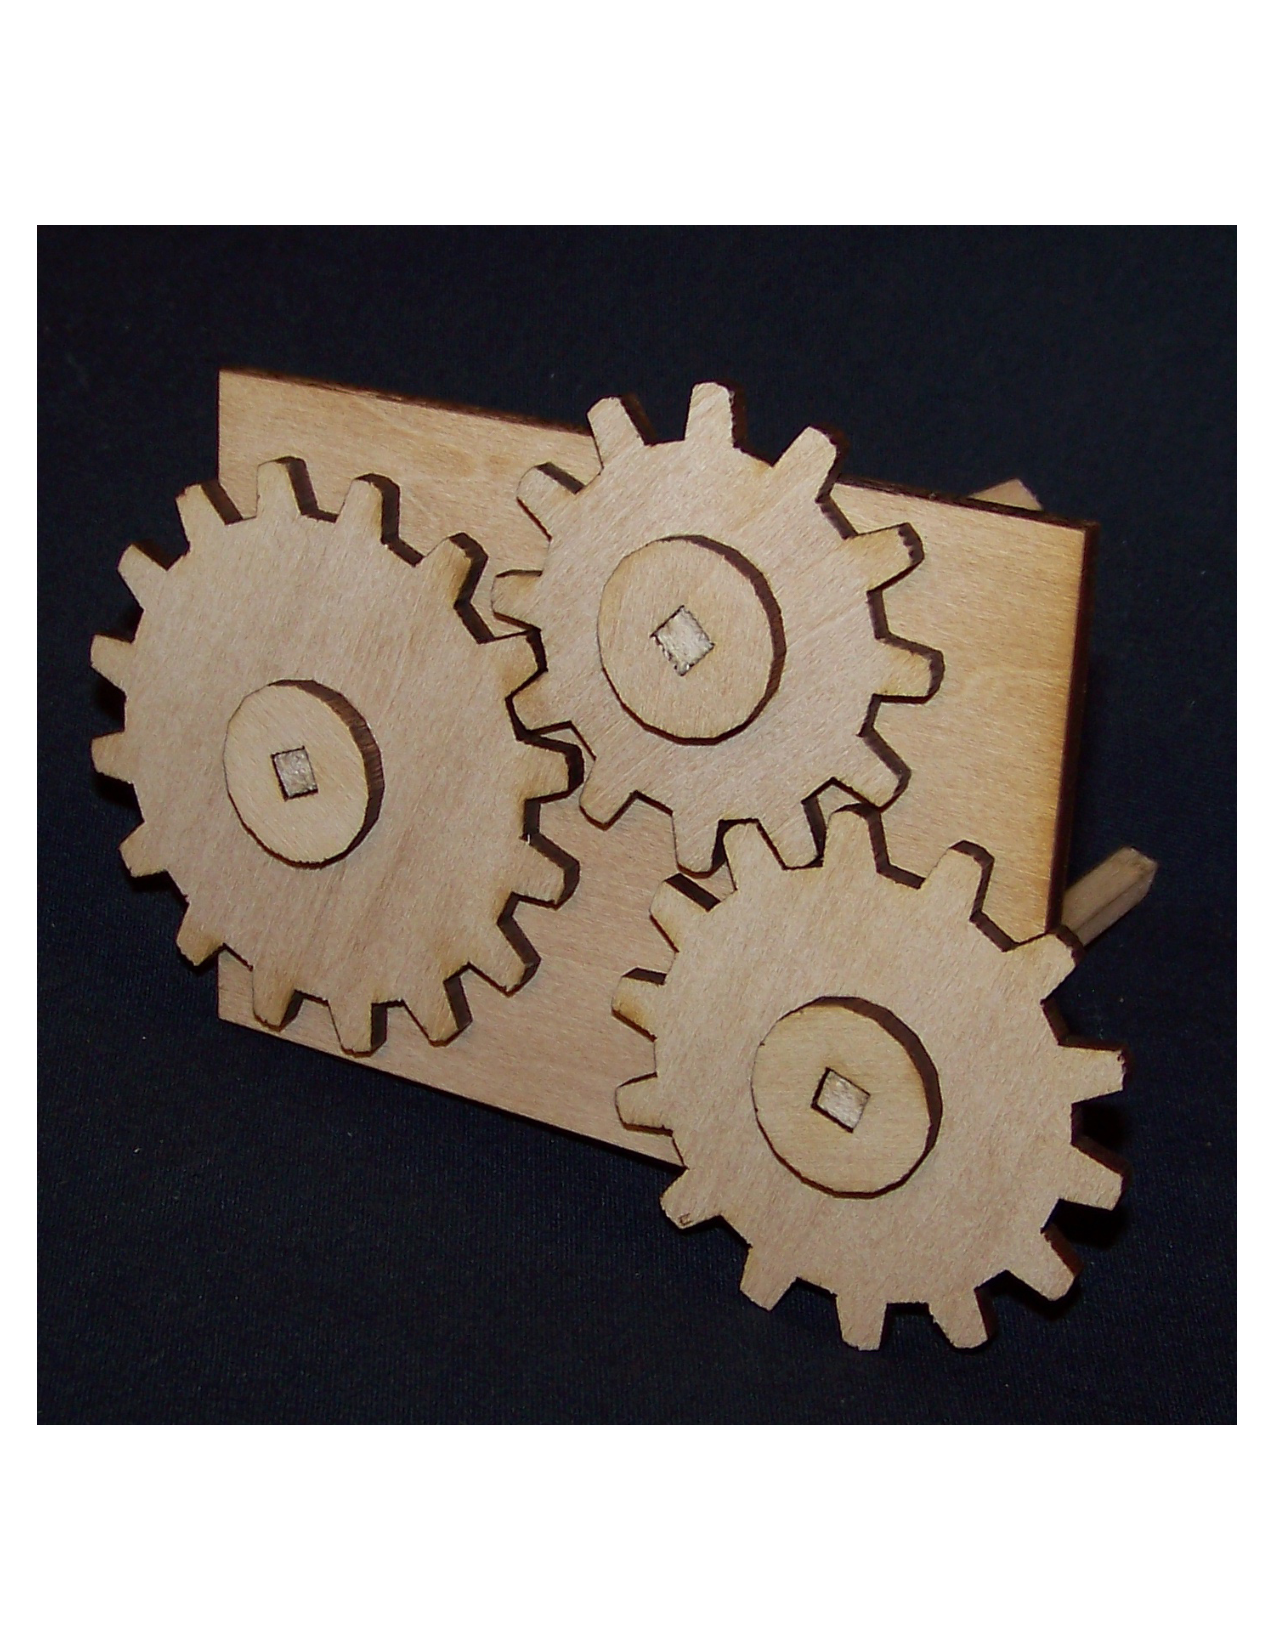
\includegraphics[width=0.9in]{physical-output-gears.pdf}
   }
   \caption{Physical output of \nohyphens{FlatCAD}.}
   \label{fig:physical-output}
\end{figure}

\section{A Mechanical Construction Kit}


\begin{figure}
\centering
  \begin{subfloat}
    \begin{minipage}{2.6in} 
      \small
\begin{verbatim}
coaxial(gear(10), piston_wheel())
link(4).draw()
\end{verbatim}
    \end{minipage}% 
  \end{subfloat} 
  \begin{minipage}{1.3in}
      \centering 
    \begin{subfloat}
      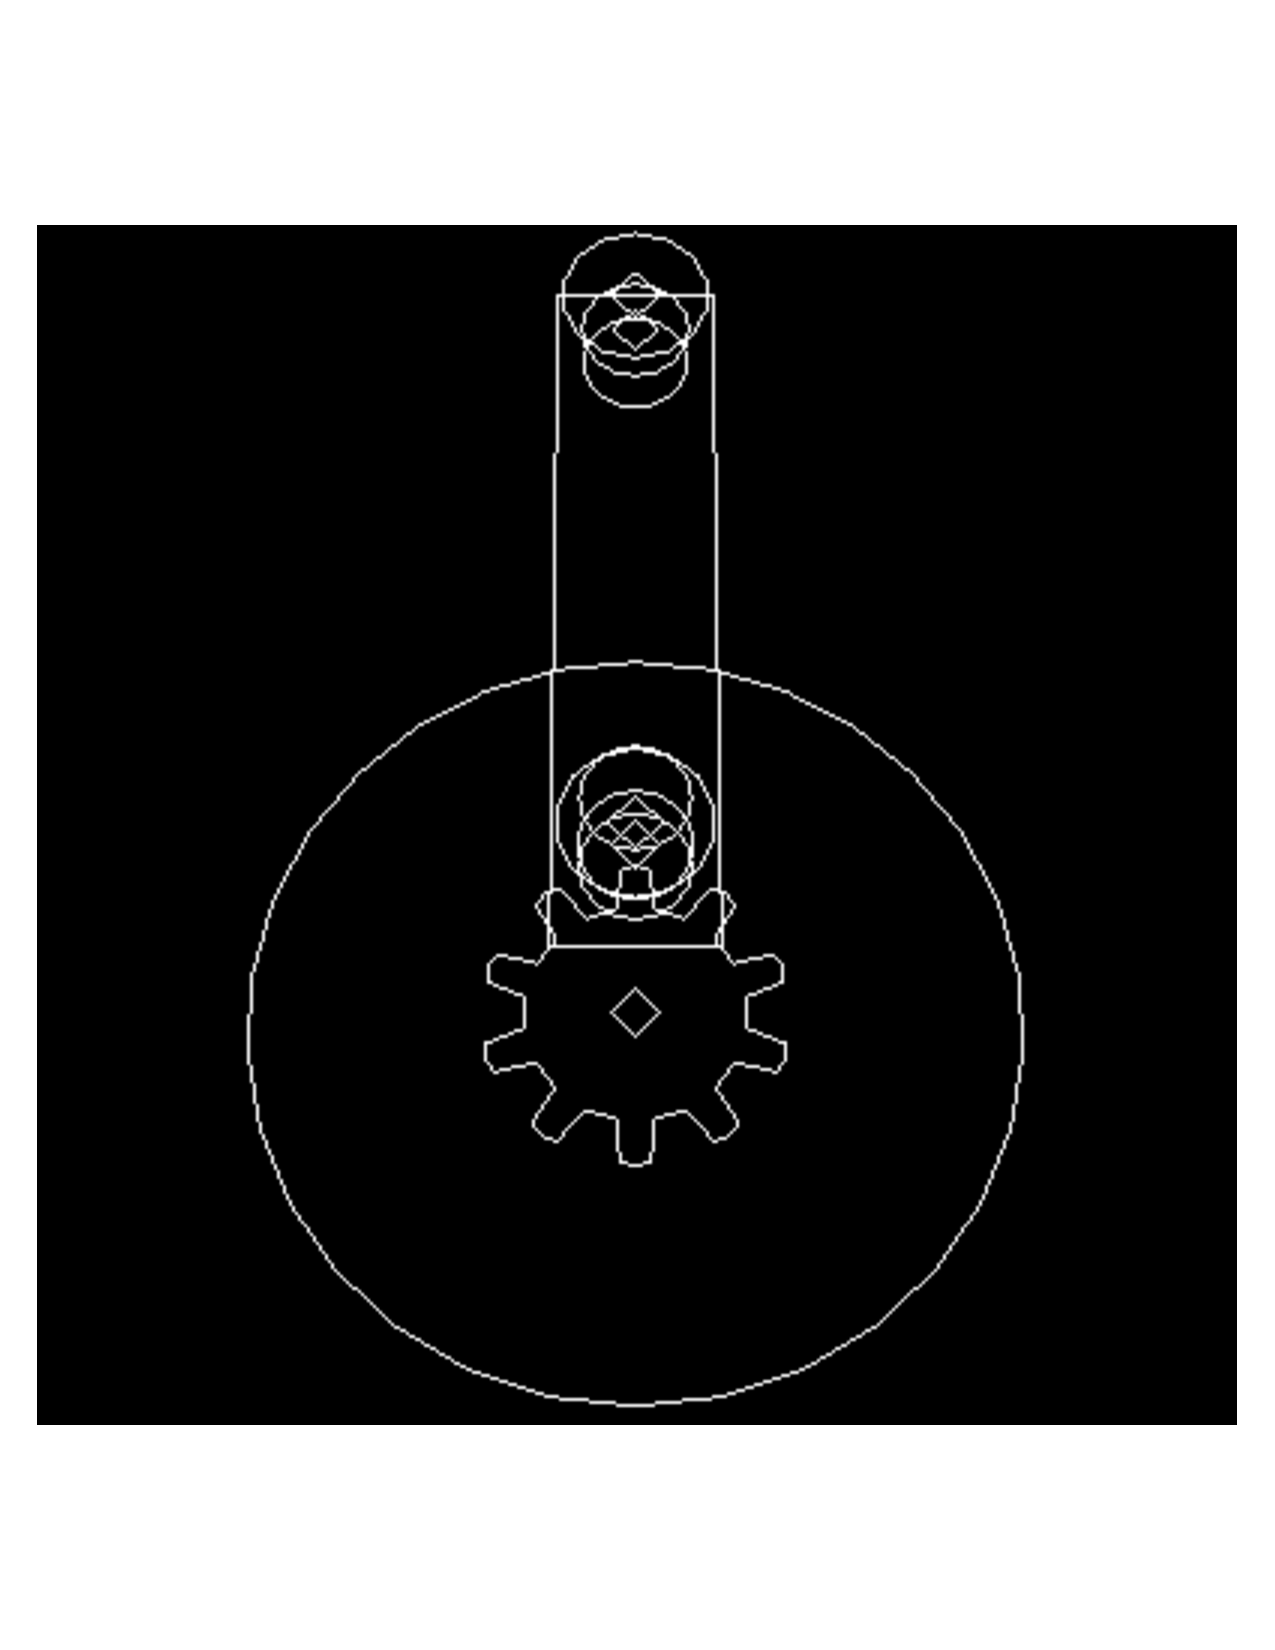
\includegraphics[width=1.3in]{mechanism_graphics.pdf}
    \end{subfloat}
  \end{minipage}
  \begin{minipage}{1.3in}
      \centering 
    \begin{subfloat}
      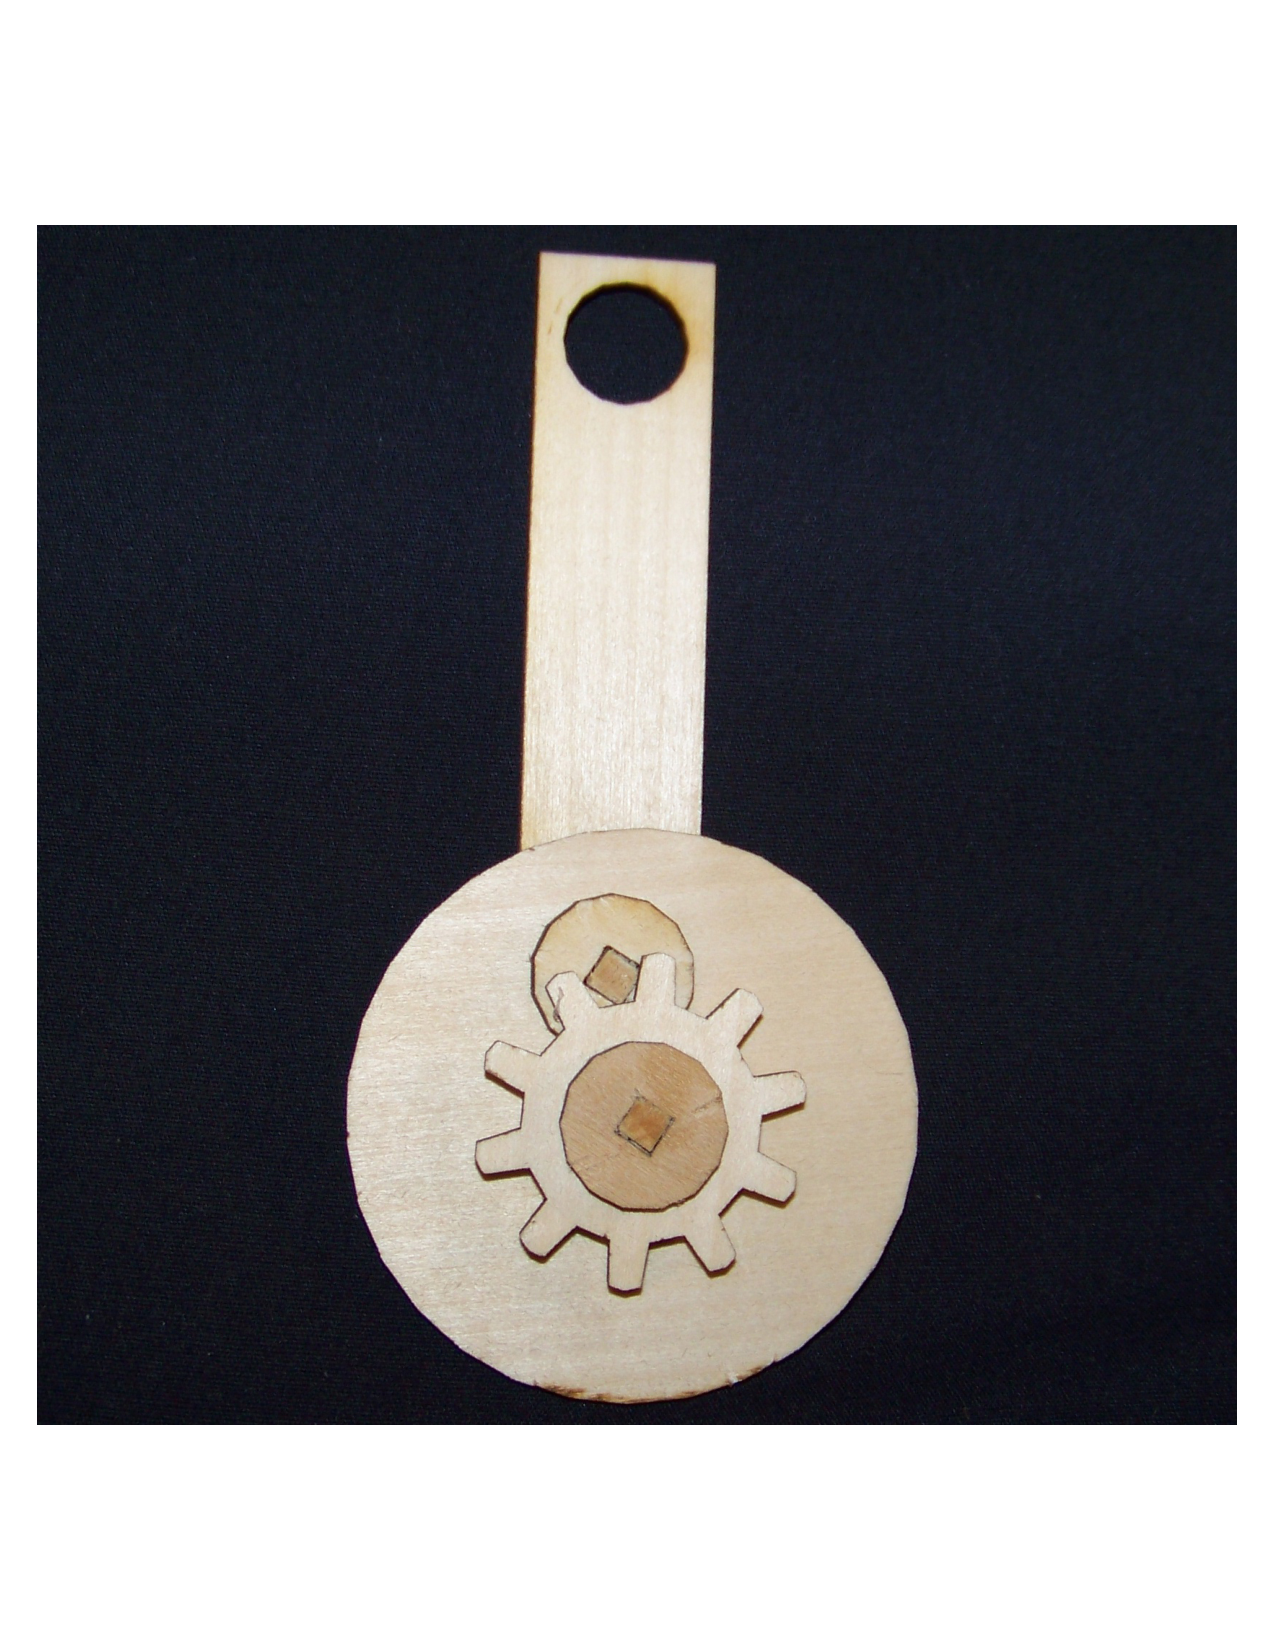
\includegraphics[width=1.3in]{mechanism_physical.pdf}
    \end{subfloat}
  \end{minipage}
  \caption{High-level \nohyphens{FlatLang} code, graphics, and
    physical output for a simple mechanism.}
  \label{fig:machine-code} 
\end{figure} 

While a physical mechanical construction kit may come with four or
five sizes of gears, a software-generated mechanical kit can render
any size gear we like. \nohyphens{FlatCAD} lets us bridge the virtual
and physical by letting us easily fabricate new models by writing
code.

Say we would like to make a toy automaton. In particular, we plan to
make a vehicle with a little puppet `driving' it. We want the puppet
to move up and down as the vehicle rolls on the floor. We must convert
the wheel's radial motion to harmonic linear motion to move the
puppet. We could build this out of existing parts (e.g. using Erector
set components), but the resulting automaton would likely not behave
exactly as we would like. Instead, we can use \nohyphens{FlatCAD} to
assemble and customize parts using a library of parametric
construction kit pieces. This lets us make exactly what we want.

One way of converting from angular to linear motion is by using a
piston wheel, like the one shown in Figure~\ref{fig:machine-code}. It
has an off-center axle attached to a rigid strut. When the other end
of the strut is constrained to move along a straight path, rotating
the wheel causes the strut to move back and forth linearly. A program
expressing this mechanism is shown in Figure~\ref{fig:automaton}.

\begin{figure}
  \begin{subfloat}
    \begin{minipage}{2.6in}
      \small
\begin{verbatim}
; wheel -- piston_wheel -- wheel
;              |
;            strut
;              |
;            puppet
;
wheel_1 = wheel()
wheel_2 = wheel()
piston = piston_wheel()
strut = link()
piston.offcenter_object = strut

coaxial(wheel_1, piston, wheel_2)
\end{verbatim}
    \end{minipage}
  \end{subfloat}
  \caption{A mechanism for a toy automaton using default dimensions
    and angles.}
  \label{fig:automaton}
\end{figure}

The mechanism resulting from the program in Figure~\ref{fig:automaton}
will move the puppet, but its speed and the amount of displacement are
constant because uses default values. We can parameterize and
customize our automaton by modifying the program. For example,
changing the value of the wheel's \textnhtt{radius} member variable
changes the puppet's up-and-down frequency. If we add gears, we can
change the puppet's speed in relation to the forward motion of the
vehicle. If we lengthen the distance between the piston wheel center
and it's off-center axle, the puppet's vertical displacement will be
greater. A revised version of this program is shown in
Figure~\ref{fig:automaton-parameteric}.

Of course, a finished toy automaton consists of more than
mechanisms. We need a chassis to hold the wheels and moving parts,
which we can make by augmenting the program further. By changing a few
parameters we may easily produce the parts list for an entire class of
toys.

\begin{figure}
  \begin{subfloat}
    \begin{minipage}{2.6in}
      \small
\begin{verbatim}
; wheel -- gear -- wheel
;           |
;          gear
;           |
;      piston_wheel
;           |
;         strut
;           |
;         puppet
;
define parametric_automaton
  (g1_teeth, g2_teeth, offset)

  wheel_1 = wheel()
  wheel_2 = wheel()
  gear_1 = gear(g1_teeth)
  gear_2 = gear(g2_teeth)
  piston = piston_wheel(offset)
  strut = link()
  piston.offcenter_object = strut

  coaxial(wheel_1, mesh(gear_1, 
          coaxial(gear_2, piston_wheel)), 
          wheel_2)
done
\end{verbatim}
    \end{minipage}
  \end{subfloat}
  \caption{A parametric version of the previous automaton.}
  \label{fig:automaton-parameteric}
\end{figure}

\section{Why Not Use Illustrator?}

% This section should head off questions about why we would use
% FlatCAD and not [Illustrator | GenerativeComponents | MEL |
% SolidWorks].

Typically people use commercial design software to make models to
produce on a laser cutter. One might ask, ``If your goal is to make
toys on a laser cutter, why not use Illustrator?''  After all,
professional designers use commercial systems all the time with much
success. The answer is that algorithmic generation of form can be
incredibly powerful. A designer may construct a few versions of the
same artifact using a traditional approach. Alternately, the designer
could write a program that is capable of generating hundreds or
thousands of variations. Instead of editing a model directly to
develop a new variation, alternatives may be generated quickly simply
by changing parameters.

Commercial design systems let designers manually specify exact
dimensions and angles. But models can also be created or edited
programmatically. For example, \nohyphens{SolidWorks} lets designers
establish constraints such as ``X is halfway between A and
B''---regardless of how A or B are manipulated, the system ensures
that X is between them. Modeling programs such as Maya or SketchUp
provide scripting capabilities so users can write programs to directly
generate or modify models.

Interaction paradigms found in these design environments can be
separated into two groups: graphical and programmatic. Some
environments offer both of these approaches, which have their own
strengths and weaknesses.

In the graphical paradigm, designers interact with the model primarily
with the mouse. This involves the designer drawing lines, selecting
and manipulating objects, or establishing relationships between
them. Here the designer can see their model in 2D or 3D as they work,
and affords direct manipulation of anything already on the screen.
% For the record, I think 'direct manipulation' is a misnomer because
% you're not directly manipulating anything. You're manipulating an
% electronic representation of something. Sorry to split hairs.

In the programming paradigm, people typically use scripts either
provided by the application developers or third parties. Occasionally
designers write their own scripts, but this requires programming
skills. Depending on the language, learning to program may be seen as
a lot of work for little payoff. Many environments use existing
general purpose languages (or variants), providing access to the GUI's
functionality via an API. For example, AutoCAD uses a variant of Lisp,
SketchUp uses Ruby, and Maya uses MEL (a scripting language bearing a
strong resemblance to Perl).

Geometry in scripting environments is usually expressed in absolute
terms. While absolute geometry is useful and powerful, it is sometimes
hard to use. For example, we may describe an object in absolute
coordinates by drawing lines from the points \textnhtt{(16.4,~2.4)},
\textnhtt{(16.4,~6.3)}, \textnhtt{(20.3,~6.3)},
\textnhtt{(20.3,~2.4)}, and \textnhtt{(16.4,~2.4)}. To a human, it is
less than clear that this representation specifies a square whose
sides are 3.9 units long. If our goal is to draw a square, we can do
this using turtle geometry by drawing a line, turning 90 degrees, and
repeating that three times. Turtle geometry is often much easier to
understand. \nohyphens{FlatCAD} lets programmers use either absolute
or differential geometry, depending on which is more appropriate.

In the previously mentioned commercial tools, programming is
supplemental to the primary graphical mode of interaction. In
\nohyphens{FlatCAD}, programming is primary mode of interaction. It
may be theoretically possible for any of these languages to do the
same things. However, from the perspective of a human designer, there
may be a significant difference between the expressive power of one
language over another. \nohyphens{FlatLang} explicitly supports people
to develop models for production on rapid prototyping machines.  The
language and the small set of built-in functions allow a designer to
quickly model physical parts and systems of parts.

\section{Related Work}

The LOGO language provides a ``microworld'' to explore programming
\cite{papert-mindstorms}. While LOGO is a complete programming
language that works without graphics, it is particularly known for the
ease that novice programmers can make visual output. LOGO's graphics
are generated with the use of two-dimensional ``turtle geometry''
\cite{abelson-turtle-geometry}, where graphics are drawn by
instructions an on-screen ``turtle'' to move or turn various
amounts. A recent LOGO-like language called FormWriter used a ``flying
turtle'' that operated in 3D \cite{gross-formwriter}. In addition to
drawing lines, FormWriter had primitive drawing functions for creating
3D objects such as cones, cylinders, and boxes. 

Programming can be an expressive medium for creative expression beyond
physical shape. For example, music and sound can be composed by
programming in Nyquist, a variant of Lisp \cite{dannenberg-nyquist}.

Triskit pieces are simple wafer-like sheets cut from acrylic sheets
and fit together at the edges with finger joints
\cite{martin-triskit}. Users can design new Triskit pieces with
arbitrary dimensions using a Java applet. The Furniture Factory and
the Designosaur capture freehand sketch input that is used to generate
dollhouse furniture and wooden dinosaur skeletons, respectively
\cite{oh-fab}. Mori and Igarashi's Plushie system lets people design
and sew plush toys \cite{mori-plushie}. Plushie offers a sketch-based,
interactive environment that generates fabric patterns that can then
be printed and sewn.

The MachineShop lets users design moving mechanical systems such as
toy automata, made from parts like gears and cams
\cite{blauvelt-automata}. Rather than directly editing the parameters
or shape of such components, MachineShop users indicate behavioral
qualities such as the distance a cam follower moves as the cam
rotates. The design tool then generates a cam providing the desired
behavior. In contrast, \nohyphens{FlatLang} programs do not reverse
engineer physical shape based on desired behavior.

\section{\nohyphens{FlatLang} Programming}

\nohyphens{FlatLang} is a dynamically typed, interpreted language. The
interpreter is written in Java, using ANTLR \cite{parr-antlr} to parse
\nohyphens{FlatLang} source code. Its syntax resembles Python's,
though indentation is not significant. Execution begins at the top of
input and proceeds from there--no \textnhtt{main()} function is
required as in C or Java.

Figure~\ref{fig:pentahedron} shows a simple \nohyphens{FlatLang}
program for making a pentahedron. In this example, the
\textnhtt{dihedralAngle} is declared and initialized to
125$^\circ$. The variable is implicitly numeric. Next, the code
declares two functions. \textnhtt{triangle} produces an equilateral
triangle of parametric size. The \textnhtt{goNext} routine `rolls' and
positions the turtle for the next operation. The end of the code
sample loops four times, explicitly creating four of the five faces of
our square pyramid. The fifth face (the base of the pyramid) was
created implicitly from the turtle's path.

\begin{figure} 
  \centering 
  \begin{subfloat}% 
    \begin{minipage}{1.8in} 
      \small
\begin{verbatim}
dihedralAngle = 125

define triangle(size)
  repeat(3)
    forward(size)
    left(120)
  done
done

define goNext(size)
  roll(-dihedralAngle)
  forward(size)
  right(90)
  roll(dihedralAngle)
done

define pentahedron()
  roll(dihedralAngle)
  repeat(4)
    triangle(3)
    goNext(3)
  done
done
\end{verbatim}

    \end{minipage}% 
  \end{subfloat} 
  \begin{minipage}{1.0in}
    \begin{subfloat}
      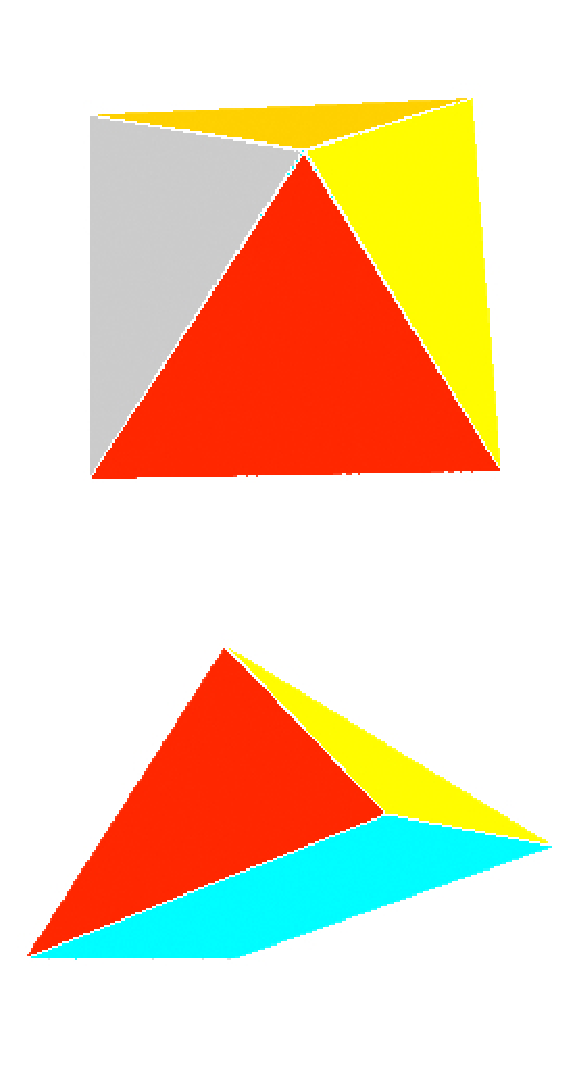
\includegraphics[width=1.0in]{pentahedron.pdf}
    \end{subfloat}
  \end{minipage}
  \caption{Low-level \nohyphens{FlatLang} code and graphics for a
    pentahedron, shown from two perspectives.}
    \label{fig:pentahedron}
\end{figure} 

While low-level \nohyphens{FlatLang} code such as the pentahedron uses
basic operations that control the turtle (like \textnhtt{forward},
\textnhtt{left} and \textnhtt{roll}), high-level \nohyphens{FlatLang}
lets us write commands to generate complex objects subject to one-way
constraints.

We have used \nohyphens{FlatLang} to develop a set of parametric
mechanical parts such as gears, piston wheels and n-bar linkages. To
facilitate assembly, we have also developed ways to express how the
parts relate. For example we may write
\textnhtt{coaxial(gear(12),~gear(24))} to make two gears that share an
axis, where one gear has twelve teeth and the other with twice that
number. Figure~\ref{fig:machine-code} shows a short
\nohyphens{FlatLang} program for part of a mechanical system capable
of driving a toy automata.

\nohyphens{FlatLang} models are intended to be `printed' using rapid
prototyping machines. The appearance on the screen is different from
the format used by computer-controlled fabrication machines like laser
cutters. The on-screen representation shows how parts relate---the
gear and piston wheel's centers are at the same location in
Figure~\ref{fig:machine-code}. However, when this is sent to a laser
cutter, those parts must be separated and arranged to make reasonably
efficient use of material. \nohyphens{FlatLang} provides the
\textnhtt{part} command to begin a new logical collection of lines
that are kept together when printing, but has no effect on the screen
representation. This lets the programmer focus on creating systems of
parts without manually separating them on the screen.

\subsection{Turtle Tree}

\nohyphens{FlatCAD} records the turtle's activity in a data structure
called the \textit{Turtle Tree}. The nodes of the tree are turtle
operations. A cursor stores the `current insertion location' that
serves as the parent of the next operation.

There are three kinds of turtle operations: geometry, pen, and naming
commands. Each operation is represented as a node in a tree
structure. Geometry commands modify the turtle's position or heading
(e.g. \textnhtt{forward}, \textnhtt{left}, \textnhtt{roll}, and
\textnhtt{pitch}). Pen commands (\textnhtt{up} and \textnhtt{down})
turn off and on the visual trail left behind when the turtle
moves. Geometry and pen nodes may have at most one child node. Named
nodes are inserted into the turtle tree with the \textnhtt{mark(s)}
function. Figure~\ref{fig:mark} shows code that uses the
\textnhtt{mark} command. Name nodes may have any number of children.

The Turtle Tree enables us to write simpler programs than would be
necessary to achieve certain behaviors. For example, we may call a
function that creates a construction kit piece, which executes an
arbitrarily complex sequence of turtle operations. We may want to
issue commands relative to features of the piece. Turtle Trees let us
rewind to those features without needing to know the details of how
the piece was made. Instead, we may simply use a single
\nohyphens{FlatLang} command to return to a location of interest. The
following sections describe how the Turtle Tree may be used.

\subsubsection{Using named turtle nodes}

The \textnhtt{backto(s)} command sets the current insertion location
to a previously named position \textnhtt{s}. The \textnhtt{backto}
command allows designers to use subroutines that move the turtle
without understanding exactly how they
work. Figure~\ref{fig:turtle-tree} depicts a Turtle Tree after using
the \tetnhtt{backto} command.

A turtle operation inherits the location, direction, and pen state
from its parent. Named nodes store this information. When the
insertion location is changed using the \textnhtt{backto} command,
subsequent turtle operations share the parent's state as well.

\begin{figure}

  \begin{subfloat}
    \begin{minipage}{2.6in}
      \small
\begin{verbatim}
define notch(len, dep, wid, name)
  fAmt = (len / 2) - (wid / 2)
  forward (fAmt)
  left(90)
  forward (dep)
  right(90)
  forward (wid / 2)
  mark(name)
  forward (wid / 2)
  right(90)
  forward (dep)
  left(90)
  forward (fAmt)  
done
\end{verbatim}
    \end{minipage}
  \end{subfloat}

  \begin{subfloat}
    \begin{minipage}{}
      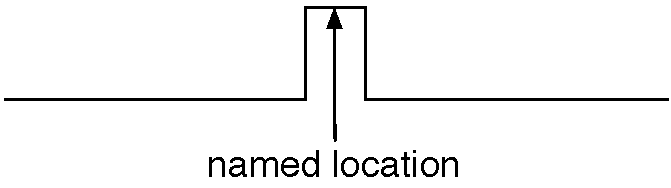
\includegraphics[width=2.0in]{notch_graphic.pdf}
    \end{minipage}
  \end{subfloat}

  \caption{A function using \textnhtt{mark} to name a feature in the
    Turtle Tree, illustrated at the bottom.}
  \label{fig:mark}
\end{figure}

\begin{figure*}
  \begin{subfloat}
    \begin{minipage}{1.6in}
      \small
\begin{verbatim}
notch(3, 0.5, 0.2, "X")
backto("X")
left(10)
notch(3, 0.5, 0.2, "Y")
\end{verbatim}
    \end{minipage}
  \end{subfloat}
  \begin{subfloat}
    \begin{minipage}{5.0in}
      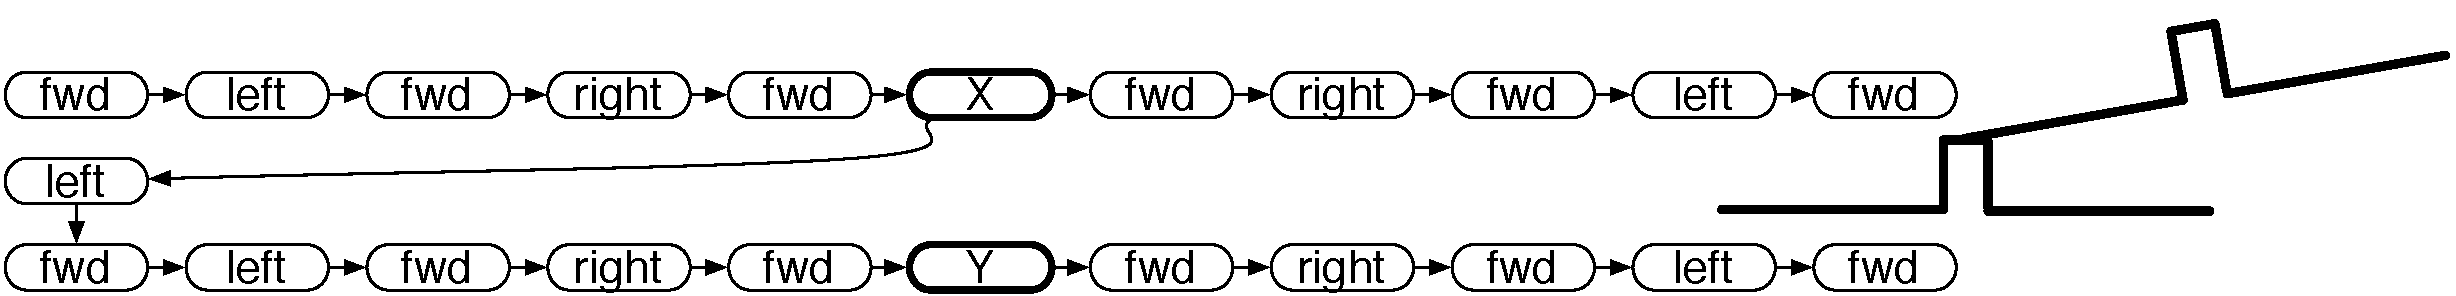
\includegraphics[width=5.0in]{turtle_tree_graph.pdf}
      \end{minipage}
  \end{subfloat}
  \caption{Code, associated Turtle Tree, and graphic output.}
  \label{fig:turtle-tree}
\end{figure*}
  


\subsubsection{Shapes}

Procedures that generate a shape typically begin and end at the same
locations. For example, the ``triangle'' function in
Figure~\ref{fig:pentahedron} always begins and ends at one corner. In
most cases this is good enough, because we may never want to draw
something in another way. However, we may want to draw a shape
beginning from one particular location, or begin drawing subsequent
parts from a different point. This commonly happens when we have a
number of parts that can fit together in many ways.

Consider the code in Figure~\ref{fig:shapes}. After the function
definitions, it creates a globally visible shape called ``tri''. The
code in the \textnhtt{shape} block is executed but it is not appended
to the model's turtle tree. Instead, \textnhtt{shape} creates a
separate circular list structure consisting of named nodes and
geometric operations. The last node added to the list refers to the
first node. We may use these named nodes as locations to begin drawing
shapes using the \textnhtt{draw} and \textnhtt{from} commands.

The \textnhtt{go} function first uses the \textnhtt{draw} command to
draw a ``tri'' shape beginning from its `a' location. This copies the
sequence of operations from the ``tri'' list to the turtle
tree. \textnhtt{draw} is helpful because it removes the need for the
designer to know exactly which sequence of turtle operations is
necessary to make the shape appear at the desired location. Next, the
\textnhtt{from} command lets us position the turtle at the bottom of
the other two notches in our triangle and draw additional pieces.

\begin{figure}

  \begin{minipage}{}
    \begin{subfloat}
      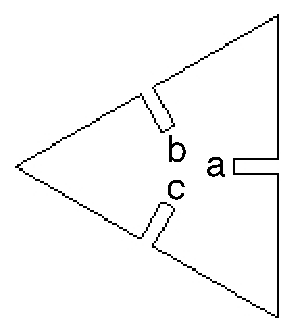
\includegraphics[width=1.2in]{notched_triangle.pdf}
      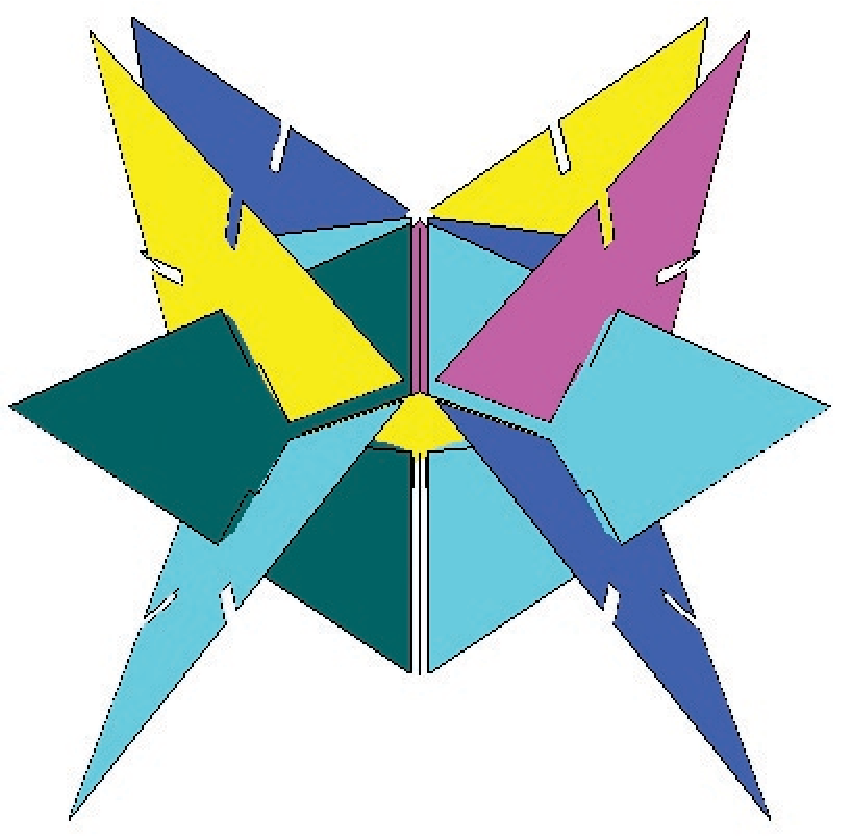
\includegraphics[width=1.8in]{shapes-complete.pdf}
    \end{subfloat}
  \end{minipage}

  \begin{subfloat}
    \begin{minipage}{2.6in}
      \small
\begin{verbatim}
define notched_tri(len, dep, wid)
  angle = 360 / 3
  notch(len, dep, wid, "a")
  left(angle)
  notch(len, dep, wid, "b")
  left(angle)
  notch(len, dep, wid, "c")
  left(angle)
done

define go(s, ttl)
  draw(s, "a")
  from("b","c")
    pitch(90)
    left(180)
    if (ttl > 0)
      go(s, ttl - 1)
    done
  done
done

shape("tri")
  notched_tri(3, 0.4, 0.1)
done

go("tri", 3)
\end{verbatim}
    \end{minipage}
  \end{subfloat}
  \caption{Recursive \nohyphens{FlatLang} code storing a shape called
    `tri', drawing it from location `a', and drawing subsequent `tri'
    shapes from locations `b' and `c'. A single `tri' is shown at top
    left, the graphic output of this program is shown at top right.}
  \label{fig:shapes}
\end{figure}

\subsubsection{Absolute geometric commands}

Most geometric turtle commands in \nohyphens{FlatLang} are interpreted
relative to the turtle's current position. Users may also use absolute
geometric commands. The \textnhtt{pos} and \textnhtt{dir} commands
return the absolute turtle position and directions. Programs may
return the turtle to previously stored positions or direction with the
\textnhtt{drawto} and \textnhtt{facedir} commands.

The absolute geometry commands are useful in cases when we are
interested in connecting points but we are not able to (or do not care
to) calculate the differential geometry between points. There are two
primary difference between the \textnhtt{mark}/\textnhtt{backto} and
\textnhtt{pos}/\textnhtt{drawto} approaches. The first is that
geometric operations inherit their pen state from their parent in the
turtle tree. While \textnhtt{backto} results in a new branch in the
turtle tree, \textnhtt{drawto} does not. Second, \textnhtt{drawto}
draws a line when the pen is down, but \textnhtt{backto} will never
draw a line.

\begin{figure}
  \begin{subfloat}
    \begin{minipage}{2.6in}
      \small
\begin{verbatim}
; make an n-sided polygon beginning and
; ending at the current turtle position.
;
define centered_polygon(sides, radius)
  angle = 360 / sides
  points = [] ; initialize empty list
  up()
  mark("middle")
  i = 0
  repeat(sides+1)
    backto("middle")
    left(i * angle)
    forward(radius)
    points = cons(pos(), points)
    i = i+1
  done
  down()
  repeat(points.n)
    p = first(points)
    points = rest(points)
    drawto(p)
  done
  backto("middle")
done
\end{verbatim}
    \end{minipage}
  \end{subfloat}
  \caption{\nohyphens{FlatLang} showing absolute and differential
    geometry as well as \textnhtt{mark} and \textnhtt{backto}.}
  \label{fig:centered_polygon}
\end{figure}

Figure~\ref{fig:centered_polygon} illustrates the use of
\textnhtt{mark}/\textnhtt{backto} and
\textnhtt{pos}/\textnhtt{drawto}. After lifting the pen up this code
marks the ``middle''. Next, vertices are calculated by rotating the
turtle counter-clockwise and moving forward. The first point is stored
twice in order to complete the tour. Next the pen is lowered, and
points are connected by repeated calls to \textnhtt{drawto}. This code
makes equilateral polygons that are exactly centered at the initial
position.

\subsection{Objects}

\nohyphens{FlatLang} lets designers make objects with instance members
and methods. There is no notion of inheritance, however. The code in
Figure~\ref{fig:collar} defines a `collar' object with two instance
variables with default values and one method. Objects provide an
abstraction and help us work at a higher level. Instead of explicitly
using turtle operations we may use object operations.

\begin{figure}
  \begin{subfloat}
    \begin{minipage}{2.6in}
      \small
\begin{verbatim}
define collar()
  c = object("collar")
  c.inner = 0.14
  c.outer = 0.4
  c.draw = collar_draw
  c
done

define collar_draw()
  part("collar")
  centered_polygon(4, inner)
  centered_polygon(14, outer)
done
\end{verbatim}
    \end{minipage}
  \end{subfloat}
  \caption{A collar object, a structural part used in a mechanical
    construction kit.}
  \label{fig:collar}
\end{figure}

\section{Discussion and Future Work}

In order to reach a wider audience, we must make the development
environment easier to use. We have begun adding support for a
debugger. Syntax highlighting in the text editor would also help find
errors.

Frequently, mechanical errors are discovered only as the parts are
physically assembled. For example, the strut attached to a piston
wheel conflicted with the wheel's structural collar. The strut could
not freely rotate. If the program had an awareness of the desired
behavior of a construction (in this case, that the strut must freely
rotate) it could provide critical feedback before users invested time
in fabricating a physical model.

It is also possible to generate models based on functional
descriptions, as in MachineShop \cite{blauvelt-automata}. For example,
desired high level description such as ``translate radial motion into
harmonic linear motion'' could be translated into \nohyphens{FlatLang}
code in a variety of ways (such as the code in
Figure~\ref{fig:automaton}). High level descriptions may be
articulated in any number of ways, such as a traditional WIMP GUI.

The primary (indeed, the only) interaction mode currently available in
\nohyphens{FlatCAD} is by programming in \nohyphens{FlatLang}. We are
interested in the possibility of presenting additional interaction
paradigms, making \nohyphens{FlatCAD} more ``equal opportunity''
\cite{cockburn-leogo} by letting users choose the appropriate mode
based on task or user preference. In particular we are interested in
recognizing freehand sketches of mechanisms and inferring behavioral
intent. This intent can then be used to generate \nohyphens{FlatLang}
code that in turn generates a functional assembly.

\section{Conclusion}

We have introduced \nohyphens{FlatCAD}, an environment for programming
physical shape. \nohyphens{FlatCAD} allows us to escape the immutable
nature of construction kit pieces by providing a straightforward way
to design and manufacture our own. The \nohyphens{FlatLang} language
offers a number of ways for working with shape, letting designers
choose the best method for the job. After designing individual parts
we can program partial or complete assemblies by describing how the
constituent parts fit together. We can see the assembly on-screen and
fabricate it using a laser cutter. The process of designing mechanisms
with code can be powerful.

\section{Acknowledgments}

This work was funded by NSF Grant ITR-0326054.

\bibliographystyle{latex8}
\bibliography{sketch-bibliography}

\end{document}  
